\documentclass[10 pt]{beamer}
\usetheme{Madrid}
\usepackage[utf8]{inputenc}
\usepackage{xspace}
\usepackage{graphicx,graphics} 
\usepackage{color}
\usepackage{amsmath}
\usepackage{amsfonts}
\usepackage{amssymb}
\usepackage{amsthm}
\usepackage{tabularx}
\usepackage{algorithm}
\usepackage{algorithmic}
\usepackage{longtable}
\usepackage{complexity}
\usepackage{tkz-graph}
\usepackage{float}
\usepackage{multicol}
\usepackage{setspace}
\usepackage[absolute,overlay]{textpos}
\graphicspath{{fig/}}

\tikzset{
  LabelStyle/.style = { rectangle, rounded corners, draw,
                       font = \bfseries },
  EdgeStyle/.append style = {-} }
\title{ Deterministic architectures for low latency in 5G and beyond systems}

\author{{\bf Maël~Guiraud}}


\institute[Nokia Bell Labs, DAVID-UVSQ] 
{
  Nokia Bell Labs France - DAVID, Universit\'e de Versailles Saint Quentin
   \\
}

\subject{Theoretical Computer Science}
\newcommand{\todo}[1]{{\color{red} TODO: {#1}}}


\begin{document}


\begin{frame}

  \titlepage
  \centering
  \includegraphics [width=25mm]{logon.png} \hspace{1cm} \includegraphics [width=17.5mm]{logod.png} \\
\end{frame}


\begin{frame}

\tableofcontents 
\end{frame}



\section{Introduction (15 min)}
\subsection{Context (5min)}
\begin{frame}{A Radio Antenna}
\begin{center}
  \includegraphics [width=\textwidth]{radio.jpg} 
\end{center}

\end{frame}
\begin{frame}{A Radio Antenna}
\begin{center}
  \includegraphics[scale=0.3]{btsppl.png}

\end{center}

\end{frame}

\begin{frame}{Radio Access Network}

\scalebox{0.4}{

\begin{tikzpicture}
  \SetGraphUnit{5}
    \tikzset{
  EdgeStyle/.append style = {->} }
   \tikzstyle{VertexStyle}=[shape = circle, draw, minimum size = 30pt]
 

  \node (p1) at (0,4) {\includegraphics[width = 1cm]{phone.png}};
 
  \node (p2) at (0,2) {\includegraphics[width = 1cm]{phone.png}};

  \node (p3) at (0,0) {\includegraphics[width = 1cm]{phone.png}};
  
   \node (r1) at (4,2) {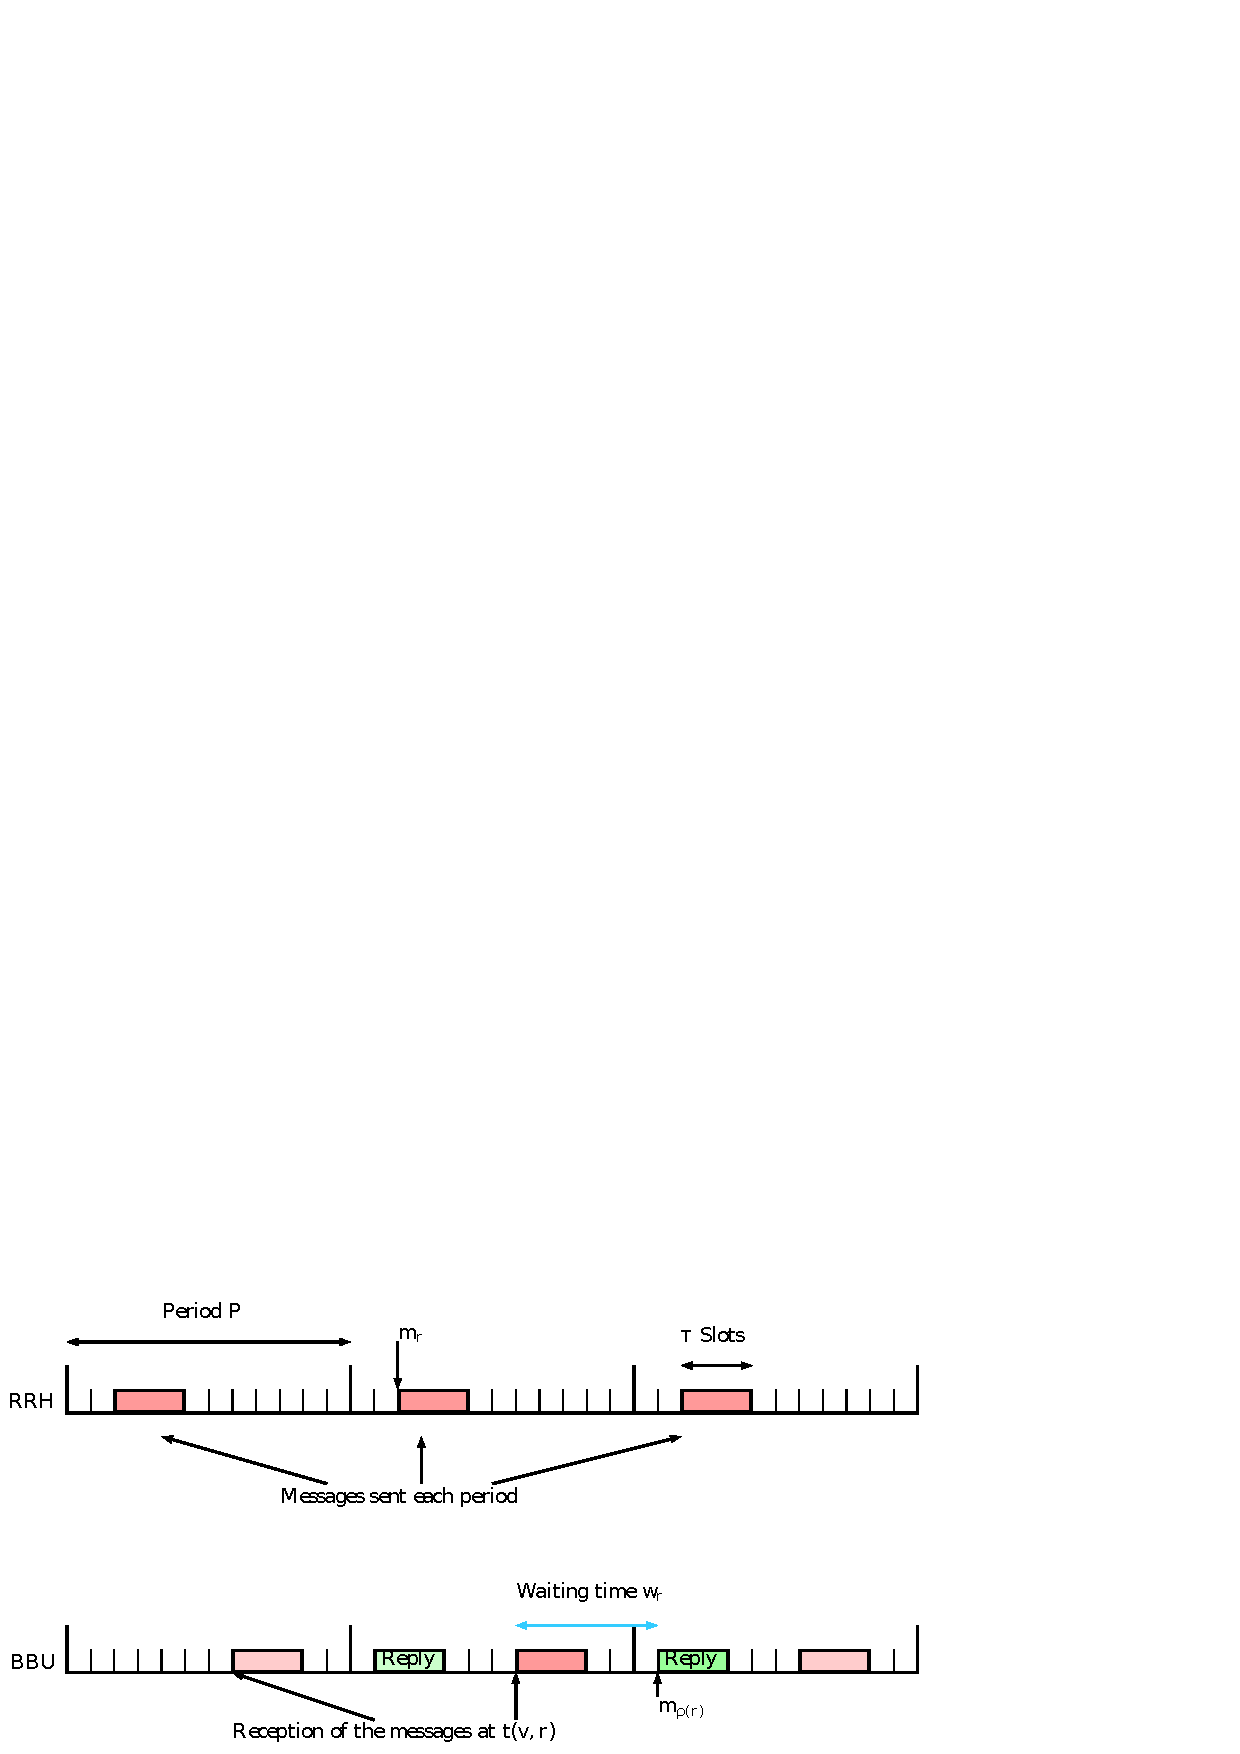
\includegraphics[width = 1cm]{rrh.png}};


 
\path (p1) edge [<->,color=red]  (r1);
\path (p2) edge [<->]  (r1);
\path (p3) edge [<->]  (r1);

\end{tikzpicture}
}


\end{frame}
\begin{frame}{Radio Access Network}

\scalebox{0.4}{

\begin{tikzpicture}
  \SetGraphUnit{5}
    \tikzset{
  EdgeStyle/.append style = {->} }
   \tikzstyle{VertexStyle}=[shape = circle, draw, minimum size = 30pt]
 

  \node (p1) at (0,4) {\includegraphics[width = 1cm]{phone.png}};
 
  \node (p2) at (0,2) {\includegraphics[width = 1cm]{phone.png}};

  \node (p3) at (0,0) {\includegraphics[width = 1cm]{phone.png}};
  
   \node (r1) at (4,2) {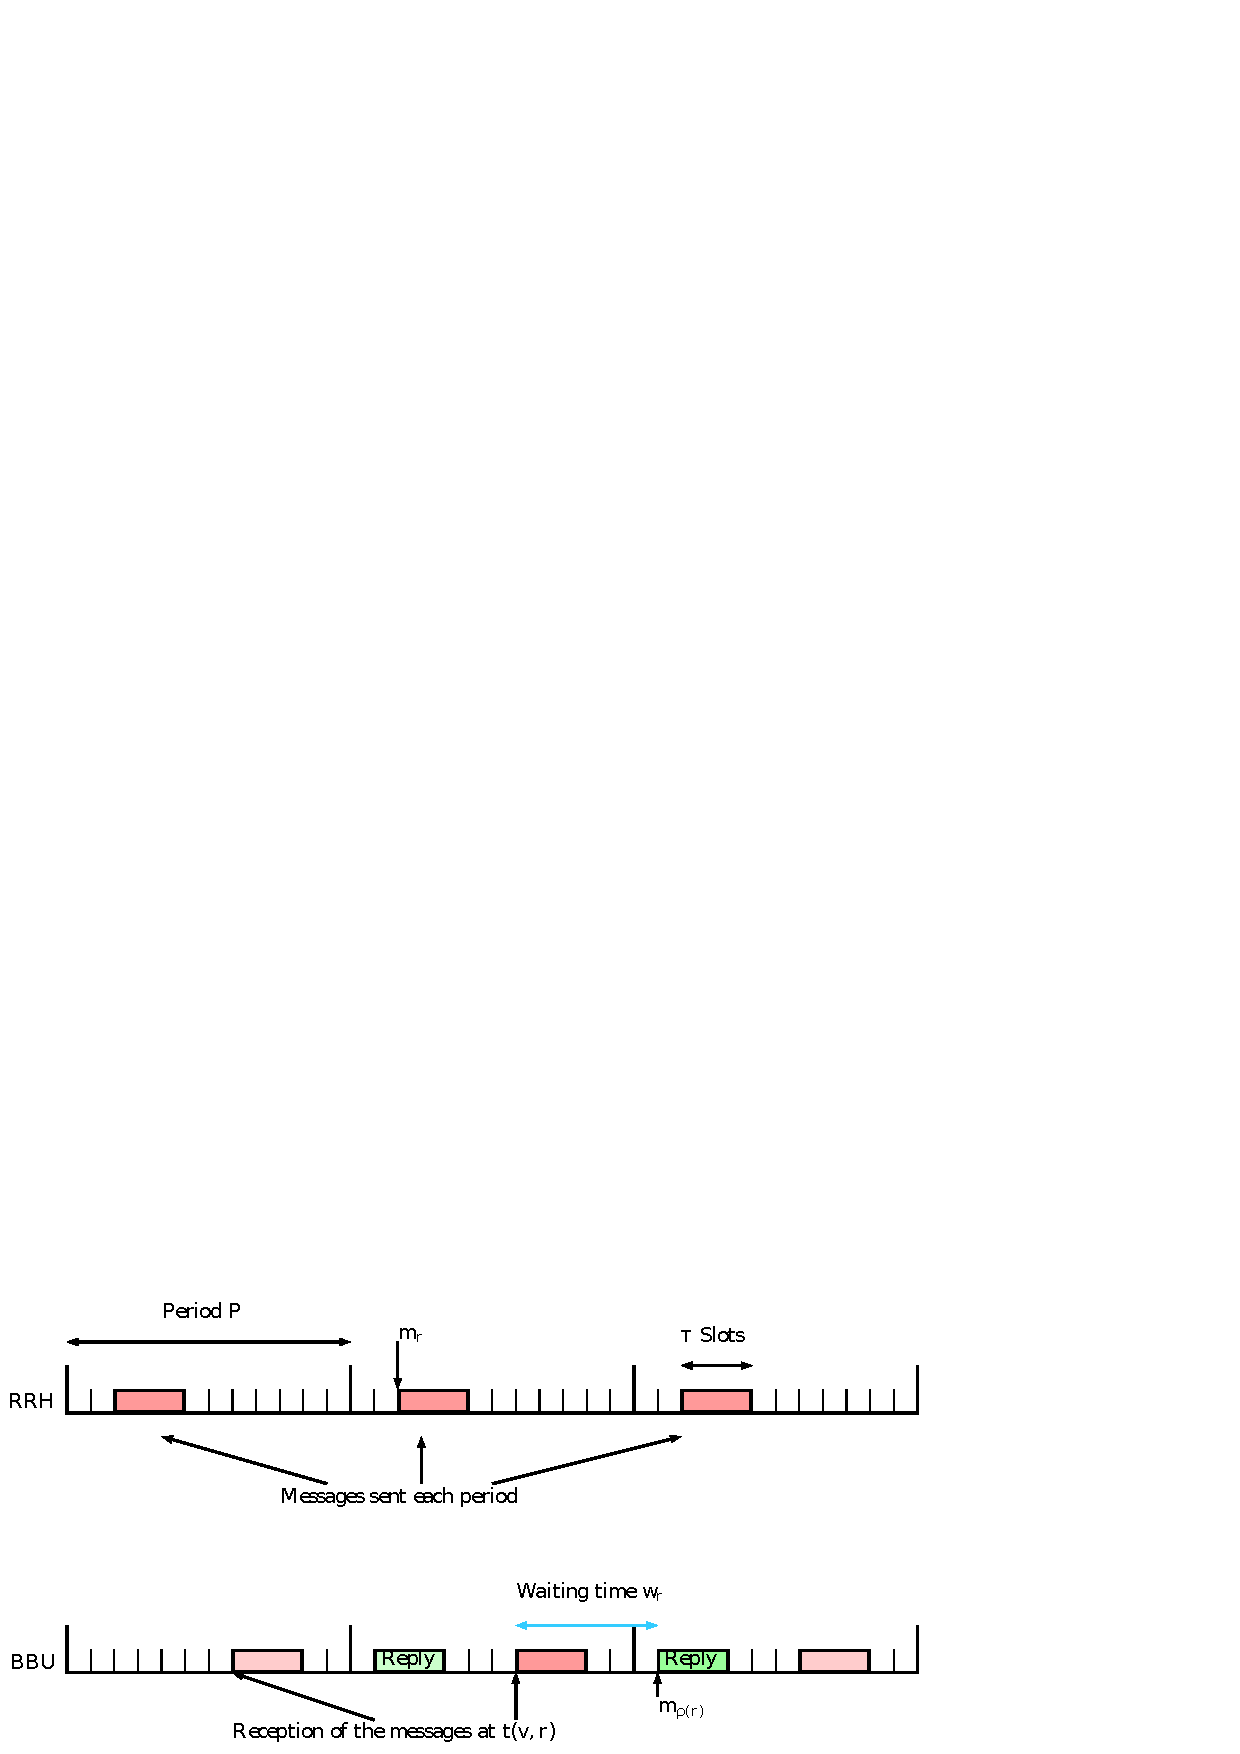
\includegraphics[width = 1cm]{rrh.png}};


 
\path (p1) edge [<->,color=red]  (r1);
\path (p2) edge [<->]  (r1);
\path (p3) edge [<->]  (r1);
\node at (3, 4) {RAN};
\end{tikzpicture}
}


\end{frame}

\begin{frame}{Aggregation network}
\scalebox{0.4}{

\begin{tikzpicture}
  \SetGraphUnit{5}
    \tikzset{
  EdgeStyle/.append style = {->} }
   \tikzstyle{VertexStyle}=[shape = circle, draw, minimum size = 30pt]
 

  \node (p1) at (0,4) {\includegraphics[width = 1cm]{phone.png}};
 
  \node (p2) at (0,2) {\includegraphics[width = 1cm]{phone.png}};

  \node (p3) at (0,0) {\includegraphics[width = 1cm]{phone.png}};
  
 \node (a1) at (7,1) {\includegraphics[width = 1cm]{switch.png}};
 \node (a2) at (7,3) {\includegraphics[width = 1cm]{switch.png}};
 \node (a3) at (9,1) {\includegraphics[width = 1cm]{switch.png}};
 \node (a4) at (9,3) {\includegraphics[width = 1cm]{switch.png}};

  
   \node (r1) at (4,2) {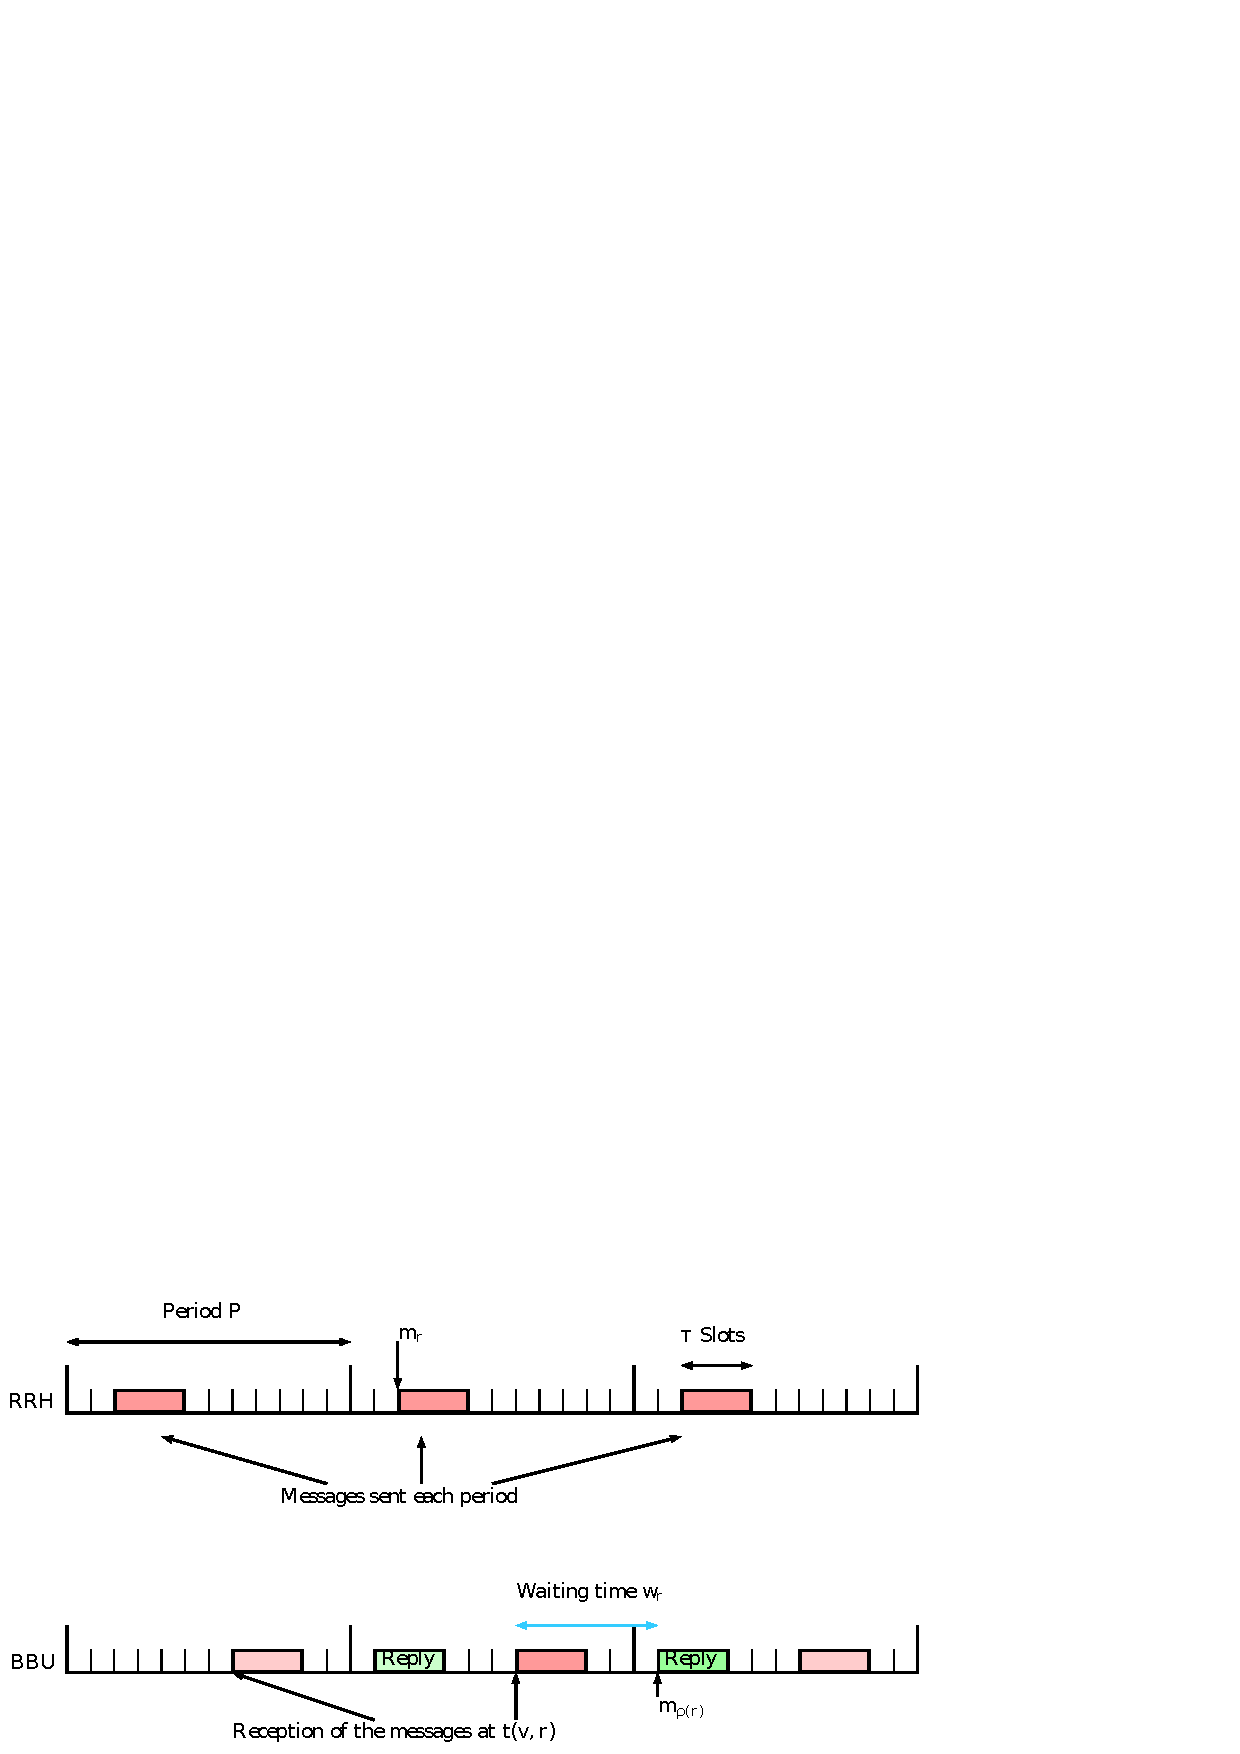
\includegraphics[width = 1cm]{rrh.png}};

   

 
\path (p1) edge [<->,color=red]  (r1);
\path (p2) edge [<->]  (r1);
\path (p3) edge [<->]  (r1);

\path (r1) edge [<->,color=red]  (a1);
\path (r1) edge [<->]  (a2);

\path (a1) edge [<->]  (a2);
\path (a3) edge [<->]  (a2);
\path (a4) edge [<->]  (a2);
\path (a3) edge [<->]  (a4);
\path (a3) edge [<->]  (a1);
\path (a4) edge [<->,color=red]  (a1);
\node at (3, 4) {RAN};


\end{tikzpicture}
}

\end{frame}


\begin{frame}{Aggregation network}
\scalebox{0.4}{

\begin{tikzpicture}
  \SetGraphUnit{5}
    \tikzset{
  EdgeStyle/.append style = {->} }
   \tikzstyle{VertexStyle}=[shape = circle, draw, minimum size = 30pt]
 

  \node (p1) at (0,4) {\includegraphics[width = 1cm]{phone.png}};
 
  \node (p2) at (0,2) {\includegraphics[width = 1cm]{phone.png}};

  \node (p3) at (0,0) {\includegraphics[width = 1cm]{phone.png}};
  
 \node (a1) at (7,1) {\includegraphics[width = 1cm]{switch.png}};
 \node (a2) at (7,3) {\includegraphics[width = 1cm]{switch.png}};
 \node (a3) at (9,1) {\includegraphics[width = 1cm]{switch.png}};
 \node (a4) at (9,3) {\includegraphics[width = 1cm]{switch.png}};

  
   \node (r1) at (4,2) {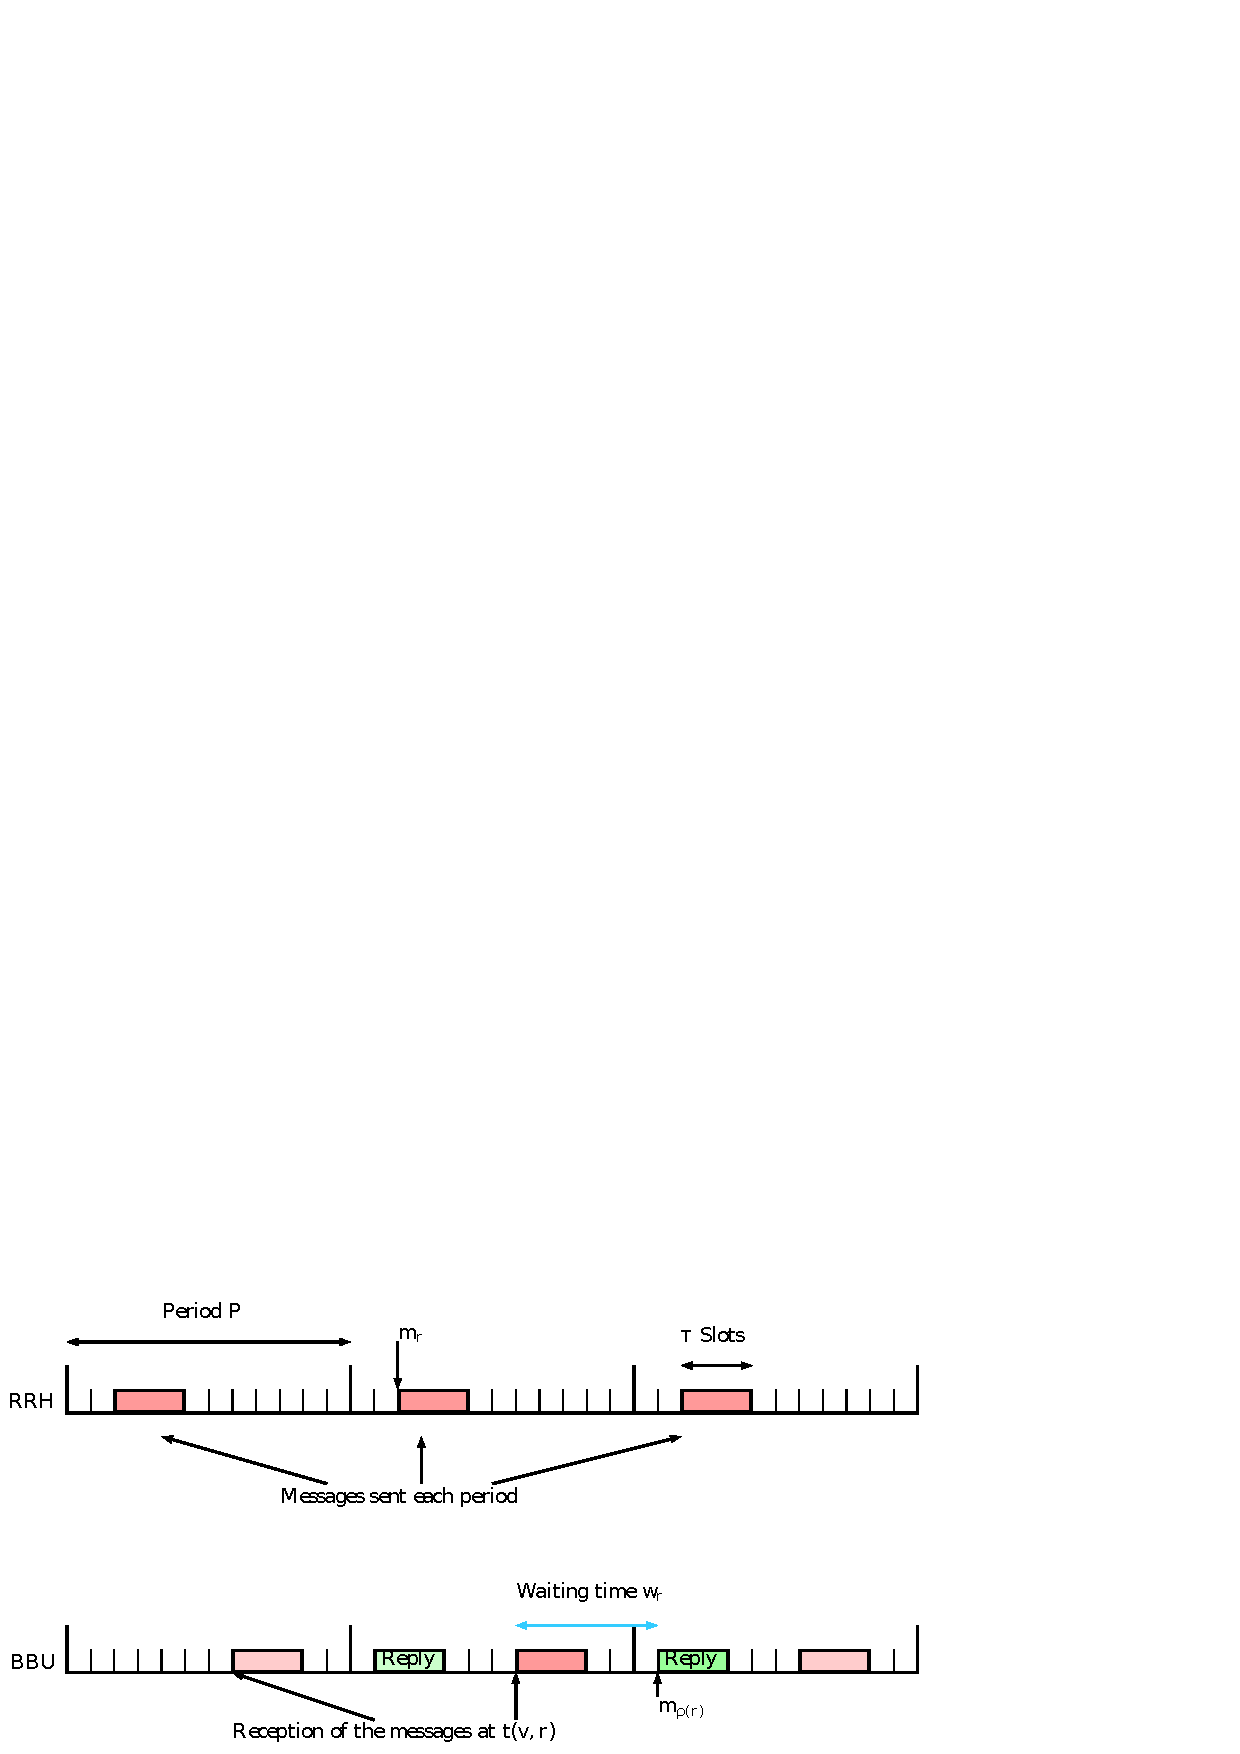
\includegraphics[width = 1cm]{rrh.png}};

   

 
\path (p1) edge [<->,color=red]  (r1);
\path (p2) edge [<->]  (r1);
\path (p3) edge [<->]  (r1);

\path (r1) edge [<->,color=red]  (a1);
\path (r1) edge [<->]  (a2);

\path (a1) edge [<->]  (a2);
\path (a3) edge [<->]  (a2);
\path (a4) edge [<->]  (a2);
\path (a3) edge [<->]  (a4);
\path (a3) edge [<->]  (a1);
\path (a4) edge [<->,color=red]  (a1);


\node at (3, 4) {RAN};
\node at (8, 4) {Aggregation};

\end{tikzpicture}
}

\end{frame}



\begin{frame}{An end-to-end communication between two terminals}
\scalebox{0.4}{

\begin{tikzpicture}
  \SetGraphUnit{5}
    \tikzset{
  EdgeStyle/.append style = {->} }
   \tikzstyle{VertexStyle}=[shape = circle, draw, minimum size = 30pt]
 

  \node (p1) at (0,4) {\includegraphics[width = 1cm]{phone.png}};
 
  \node (p2) at (0,2) {\includegraphics[width = 1cm]{phone.png}};

  \node (p3) at (0,0) {\includegraphics[width = 1cm]{phone.png}};
  
 \node (a1) at (7,1) {\includegraphics[width = 1cm]{switch.png}};
 \node (a2) at (7,3) {\includegraphics[width = 1cm]{switch.png}};
 \node (a3) at (9,1) {\includegraphics[width = 1cm]{switch.png}};
 \node (a4) at (9,3) {\includegraphics[width = 1cm]{switch.png}};

 \node (c1) at (12,3) {\includegraphics[width = 1cm]{switch.png}};
 \node (c2) at (12,5) {\includegraphics[width = 1cm]{switch.png}};
 \node (c3) at (14,3) {\includegraphics[width = 1cm]{switch.png}};
 \node (c4) at (14,5) {\includegraphics[width = 1cm]{switch.png}};

 \node (a5) at (17,1) {\includegraphics[width = 1cm]{switch.png}};
 \node (a6) at (17,3) {\includegraphics[width = 1cm]{switch.png}};
 \node (a7) at (19,1) {\includegraphics[width = 1cm]{switch.png}};
 \node (a8) at (19,3) {\includegraphics[width = 1cm]{switch.png}};


 \node (p4) at (26,4) {\includegraphics[width = 1cm]{phone.png}};
 
  \node (p5) at (26,2) {\includegraphics[width = 1cm]{phone.png}};

  \node (p6) at (26,0) {\includegraphics[width = 1cm]{phone.png}};
  
   \node (r1) at (4,2) {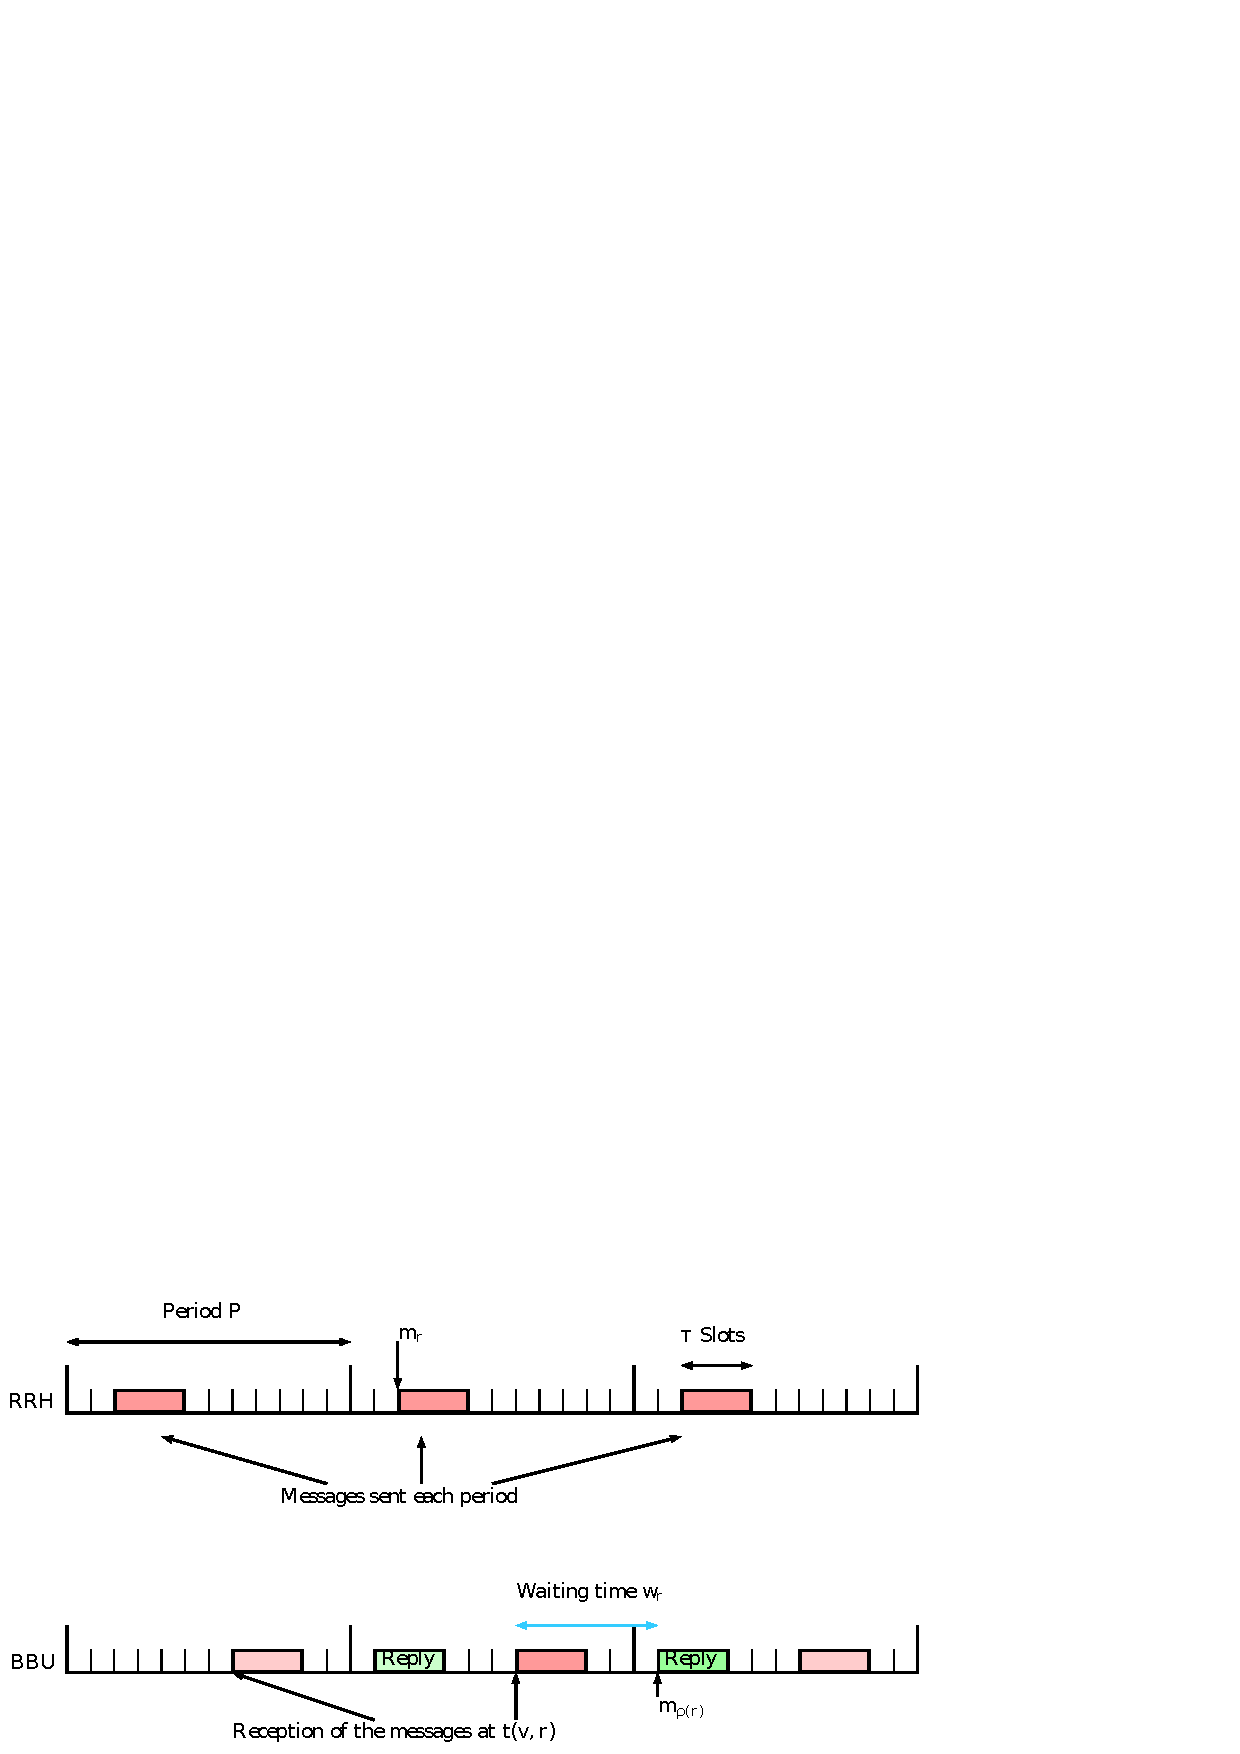
\includegraphics[width = 1cm]{rrh.png}};
   \node (r2) at (22,2) {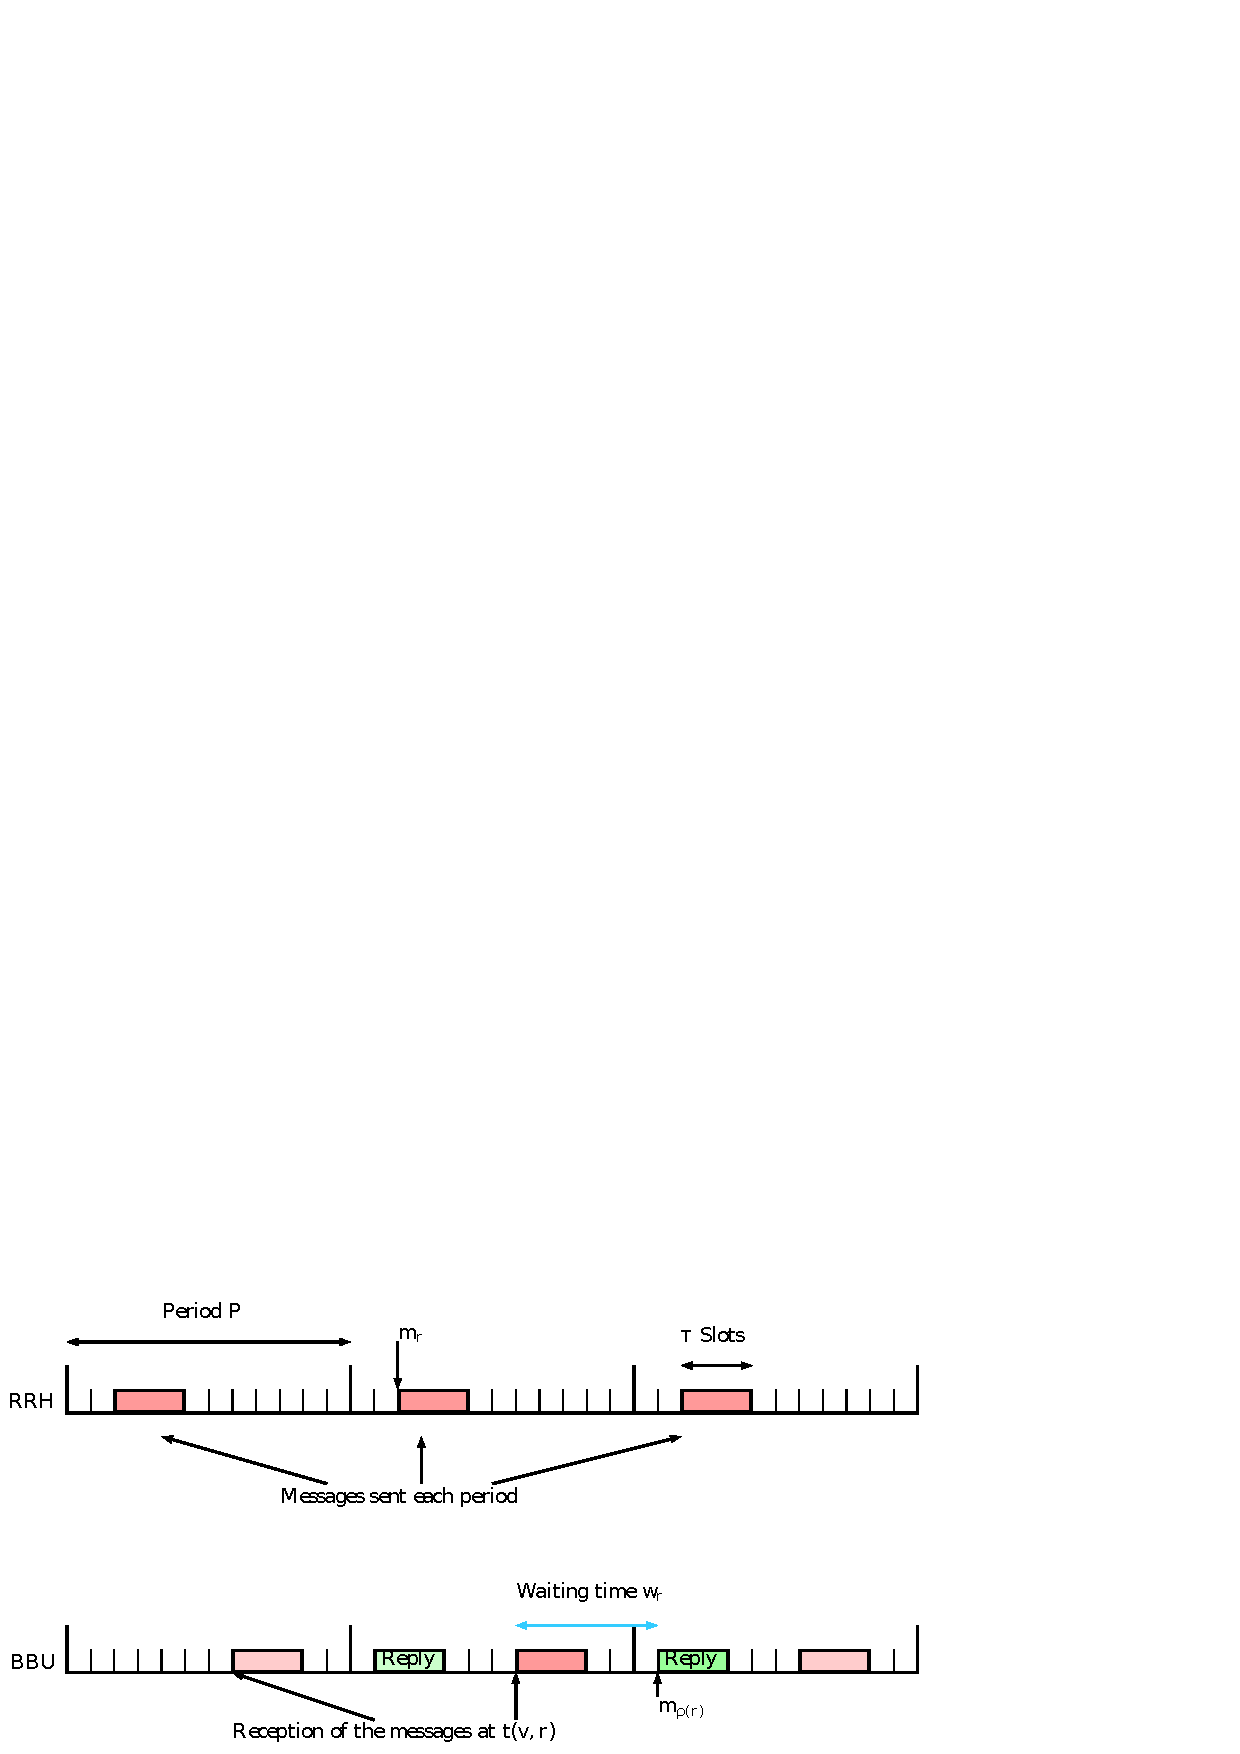
\includegraphics[width = 1cm]{rrh.png}};
   

 
\path (p1) edge [<->,color=red]  (r1);
\path (p2) edge [<->]  (r1);
\path (p3) edge [<->]  (r1);

\path (r1) edge [<->,color=red]  (a1);
\path (r1) edge [<->]  (a2);

\path (a1) edge [<->]  (a2);
\path (a3) edge [<->]  (a2);
\path (a4) edge [<->]  (a2);
\path (a3) edge [<->]  (a4);
\path (a3) edge [<->]  (a1);
\path (a4) edge [<->,color=red]  (a1);


\path (c1) edge [<->]  (c2);
\path (c3) edge [<->]  (c2);
\path (c4) edge [<->]  (c2);
\path (c3) edge [<->]  (c4);
\path (c3) edge [<->]  (c1);
\path (c4) edge [<->,color=red]  (c1);


\path (a5) edge [<->]  (a6);
\path (a7) edge [<->]  (a6);
\path (a8) edge [<->,color=red]  (a6);
\path (a7) edge [<->]  (a8);
\path (a7) edge [<->]  (a5);
\path (a8) edge [<->]  (a5);

 
\path (p4) edge [<->]  (r2);
\path (p5) edge [<->,color=red]  (r2);
\path (p6) edge [<->]  (r2);


\path (a4) edge [<->]  (c2);
\path (a3) edge [<->]  (c1);
\path (a3) edge [<->]  (c2);
\path (a4) edge [<->,color=red]  (c1);


\path (a6) edge [<->,color=red]  (c4);
\path (a5) edge [<->]  (c3);
\path (a5) edge [<->]  (c4);
\path (a6) edge [<->]  (c3);

\path (r2) edge [<->,color=red]  (a8);
\path (r2) edge [<->]  (a7);
\draw[dashed] (-1,-1) rectangle  (10,7);
\node at (3, 4) {RAN};
\node at (8, 4) {Aggregation};

\draw[dashed] (16,-1) rectangle  (27,7);
\node at (23, 4) {RAN};
\node at (18, 4) {Aggregation};

\draw[dashed] (11,2) rectangle  (15,7);
\node at (13, 6.5) {\huge Core};

\end{tikzpicture}
}

\end{frame}



\begin{frame}{What does Cloud-RAN means?}
  \centering
  \includegraphics[scale=0.2]{cloudbts.png}\\
  \includegraphics[scale=0.175]{BBURRH.png}
  
   RU=RRH, Distributed/Centralized Unit=BBU
\end{frame}



\begin{frame}{Cloud-RAN}
  \centering
  \includegraphics[scale=0.3]{CRAN}\\
  \vspace{0.5cm}
  \pause
  C-RAN aims to mutualize the computation ressources.
  
  \textcolor{red}{Since the processing time is constrained by protocol, the lower the transmission delay, the more important the sharing (ie. the coverage area of a data center).}
  
  \textcolor{blue}{The minimum latency allows to increase the mutualization.}
  
  
\end{frame}


\begin{frame}{Problematic}
  \centering
  
  
 \begin{multicols}{2}
Specificity of Cloud-RAN:
\vspace{1cm}
\begin{itemize}
\item \textcolor{red}{Minimize latency}: increase the cover area.
\item Periodic traffic 

\end{itemize}
\vspace{2cm}
Current approaches: \begin{itemize}
\vspace{1cm}
\item Dedicated network $\rightarrow$ Too expensive
\item Statistical multiplexing (TSN/Qbv) $\rightarrow$ \textcolor{red}{bounded latency only}
\end{itemize}
\end{multicols}

\end{frame}


\begin{frame}{5G Context}


  \centering
  
  \includegraphics[scale=0.4]{usecases.png}
  

\end{frame}
\begin{frame}{Other use cases}


  \centering
  
  \includegraphics[scale=0.4]{ind40.jpg}

  Industry 4.0

\end{frame}
\begin{frame}{Other use cases}


  \centering
  
  \includegraphics[scale=0.25]{vehicle.jpg}

  Autonomous Vehicle

\end{frame}

\subsection{Model, problems (10 min)}

\begin{frame}{Model}
\begin{center}
  \includegraphics [width=9cm]{1routealler} 
\end{center}

\begin{itemize}
\item Network $\rightarrow$ Weighted DAG
\item  Physical Delay of a link $\rightarrow$ Weight of the arc
\item  Only the contention points are represented in the graph
\end{itemize}

\begin{center}
\scalebox{0.6}{

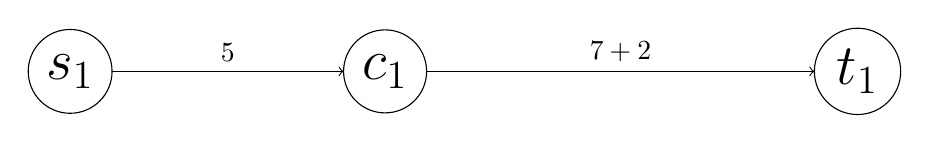
\begin{tikzpicture}
  \SetGraphUnit{5}
    \tikzset{
  EdgeStyle/.append style = {->} }
   \tikzstyle{VertexStyle}=[shape = circle, draw, minimum size = 30pt]
   \renewcommand{\VertexLightFillColor}{orange}
  \Vertex[x=0,y=0, L = {\huge $s_1$}]{s1};

\Vertex[x=10,y=0, L = {\huge $t_1$}]{t1};

  \Vertex[x=4,y=0, L = {\huge $c_1$}]{c1}
  
 %\SetVertexNoLabel
  %\Vertex[x=4,y=2]{n1}

 % \Edge[label = $5$](s1)(c1)
 % \Edge[label = $7 + 2$](c1)(t1)
  \path (s1) edge [->] node[anchor=south]{$5$} (c1);
\path (c1) edge [->] node[anchor=south]{$7+2$} (t1);

 


\end{tikzpicture}
}
  \end{center}


 \end{frame}
 
\begin{frame}{Model}
Both ways: from RRH to BBU (forward) then from BBU to RRH (backward)
 \begin{center}
  \includegraphics [width=9cm]{1routeretour} 
\end{center}


\begin{center}
\scalebox{0.6}{

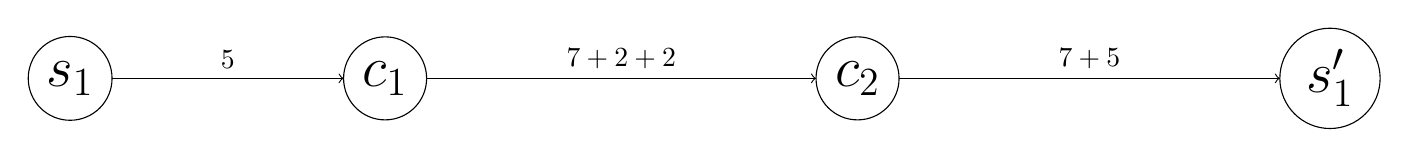
\begin{tikzpicture}
  \SetGraphUnit{5}
    \tikzset{
  EdgeStyle/.append style = {->} }
   \tikzstyle{VertexStyle}=[shape = circle, draw, minimum size = 30pt]
   \renewcommand{\VertexLightFillColor}{orange}
  \Vertex[x=0,y=0, L = {\huge $s_1$}]{s1};
\Vertex[x=16,y=0, L = {\huge $s_1'$}]{s1p};
\Vertex[x=10,y=0, L = {\huge $c_2$}]{c2};

  \Vertex[x=4,y=0, L = {\huge $c_1$}]{c1}
  
 %\SetVertexNoLabel
  %\Vertex[x=4,y=2]{n1}

  %\Edge[label = $5$](s1)(c1)
 % \Edge[label = $7 + 2+2$](c1)(c2)
 % \Edge[label = $7 + 2+2$](c1)(c2)
%\Edge[label = $7 + 5$](c2)(s1p)
 
\path (s1) edge [->] node[anchor=south]{$5$} (c1);
\path (c1) edge [->] node[anchor=south]{$7+2+2$} (c2);
\path (c2) edge [->] node[anchor=south]{$7+5$} (s1p);


\end{tikzpicture}
}
\end{center}
\end{frame}

\begin{frame}{Model}

 \begin{center}
  \includegraphics [width=7.5cm]{starfronthaul} 
\end{center}


\begin{center}
\scalebox{0.6}{

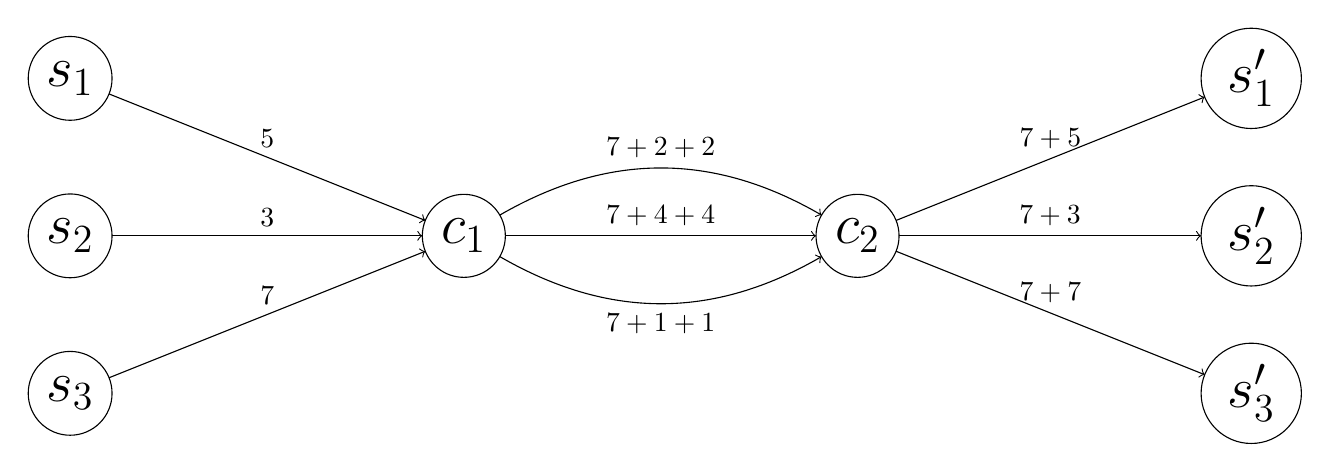
\begin{tikzpicture}
  \SetGraphUnit{5}
    \tikzset{
  EdgeStyle/.append style = {->} }
   \tikzstyle{VertexStyle}=[shape = circle, draw, minimum size = 30pt]
   \renewcommand{\VertexLightFillColor}{orange}
  \Vertex[x=0,y=4, L = {\huge $s_1$}]{s1};
  \Vertex[x=0,y=2, L = {\huge $s_2$}]{s2};
\Vertex[x=0,y=0, L = {\huge $s_3$}]{s3};
\Vertex[x=15,y=4, L = {\huge $s_1'$}]{s1p};
\Vertex[x=15,y=2, L = {\huge $s_2'$}]{s2p};
\Vertex[x=15,y=0, L = {\huge $s_3'$}]{s3p};
\Vertex[x=10,y=2, L = {\huge $c_2$}]{c2};

  \Vertex[x=5,y=2, L = {\huge $c_1$}]{c1}
  
 %\SetVertexNoLabel
  %\Vertex[x=4,y=2]{n1}

  %\Edge[label = $5$](s1)(c1)
  %\Edge[label = $7 + 4+4$](c1)(c2)
  %\Edge[label = $3$](s2)(c1)
   %\Edge[label = $7$](s3)(c1)
  %  \Edge[label = $7+3$](c2)(s2p)
 %  \Edge[label = $7+7$](c2)(s3p)
%\Edge[label = $7 + 5$](c2)(s1p)
\path (s1) edge [->] node[anchor=south]{$5$} (c1);

\path (s2) edge [->] node[anchor=south]{$3$} (c1);
\path (s3) edge [->] node[anchor=south]{$7$} (c1);
\path (c2) edge [->] node[anchor=south]{$7+3$} (s2p);
\path (c2) edge [->] node[anchor=south]{$7+7$} (s3p);

\path (c2) edge [->] node[anchor=south]{$7+5$} (s1p);

\path (c1) edge [->] node[anchor=south]{$7+4+4$} (c2);

\path (c1) edge [->,bend left=30] node[anchor=south]{$7+2+2$} (c2);
\path (c1) edge [->,bend right=30] node[anchor=north]{$7+1+1$} (c2);

  %\draw[->,line width=0.5pt] (5,2.51) parabola bend (7.5,3.5) (10,2.51);
 %\draw[->,line width=0.5pt] (5,1.49) parabola bend (7.5,0.5) (10,1.49);
 

\end{tikzpicture}
}
\end{center}
\end{frame}
  \begin{frame}{The communication process}
 
 \begin{center}
\scalebox{0.3}{

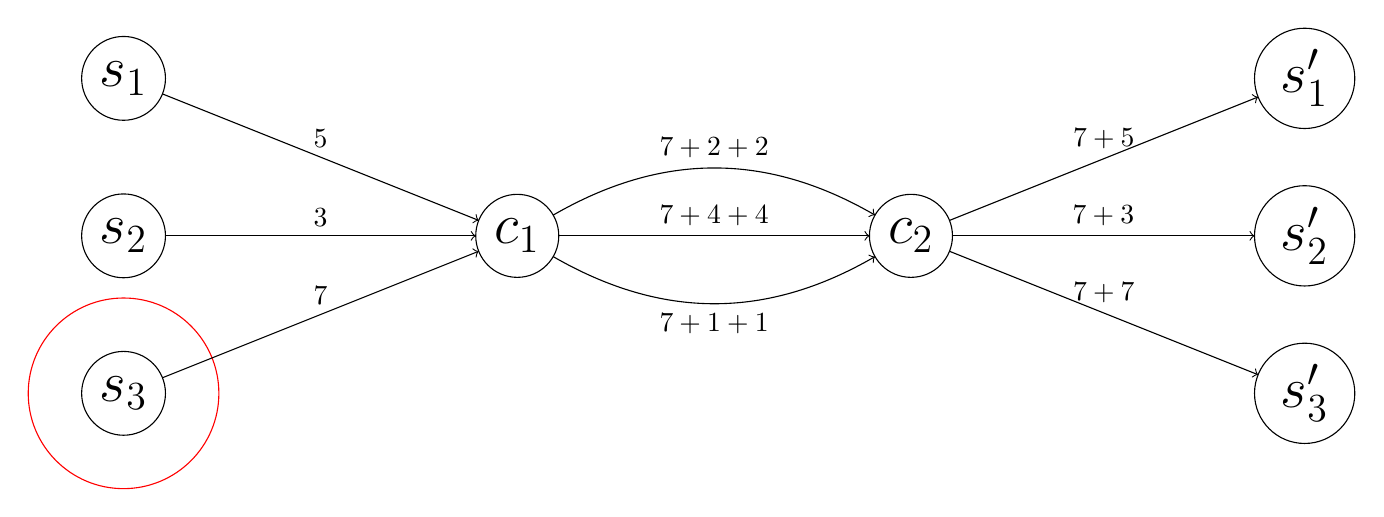
\begin{tikzpicture}
  \SetGraphUnit{5}
    \tikzset{
  EdgeStyle/.append style = {->} }
   \tikzstyle{VertexStyle}=[shape = circle, draw, minimum size = 30pt]
   \renewcommand{\VertexLightFillColor}{orange}
  \Vertex[x=0,y=4, L = {\huge $s_1$}]{s1};
  \Vertex[x=0,y=2, L = {\huge $s_2$}]{s2};
\Vertex[x=0,y=0, L = {\huge $s_3$}]{s3};
\Vertex[x=15,y=4, L = {\huge $s_1'$}]{s1p};
\Vertex[x=15,y=2, L = {\huge $s_2'$}]{s2p};
\Vertex[x=15,y=0, L = {\huge $s_3'$}]{s3p};
\draw[red] (0,0) circle (8ex);
\Vertex[x=10,y=2, L = {\huge $c_2$}]{c2};

  \Vertex[x=5,y=2, L = {\huge $c_1$}]{c1}
  
 %\SetVertexNoLabel
  %\Vertex[x=4,y=2]{n1}

  %\Edge[label = $5$](s1)(c1)
  %\Edge[label = $7 + 4+4$](c1)(c2)
  %\Edge[label = $3$](s2)(c1)
   %\Edge[label = $7$](s3)(c1)
  %  \Edge[label = $7+3$](c2)(s2p)
 %  \Edge[label = $7+7$](c2)(s3p)
%\Edge[label = $7 + 5$](c2)(s1p)
\path (s1) edge [->] node[anchor=south]{$5$} (c1);

\path (s2) edge [->] node[anchor=south]{$3$} (c1);
\path (s3) edge [->] node[anchor=south]{$7$} (c1);
\path (c2) edge [->] node[anchor=south]{$7+3$} (s2p);
\path (c2) edge [->] node[anchor=south]{$7+7$} (s3p);

\path (c2) edge [->] node[anchor=south]{$7+5$} (s1p);

\path (c1) edge [->] node[anchor=south]{$7+4+4$} (c2);

\path (c1) edge [->,bend left=30] node[anchor=south]{$7+2+2$} (c2);
\path (c1) edge [->,bend right=30] node[anchor=north]{$7+1+1$} (c2);

  %\draw[->,line width=0.5pt] (5,2.51) parabola bend (7.5,3.5) (10,2.51);
 %\draw[->,line width=0.5pt] (5,1.49) parabola bend (7.5,0.5) (10,1.49);
 

\end{tikzpicture}
}
\end{center}
\pause
\begin{center}
  \includegraphics [width=11.5cm]{rrhtime} 
  \end{center}
 \vspace{0.5cm}
   
   Every $P$ units of time, a message of size $\tau$ is emitted from each RRH.
$P$ and $\tau$ are fixed by the context. 
\pause
   The process is \textcolor{red}{periodic} : the message is emitted in each period at the same time, called \textcolor{blue}{offset}.
   
\end{frame}


 \begin{frame}{Collisions}

\begin{center}
\scalebox{0.6}{

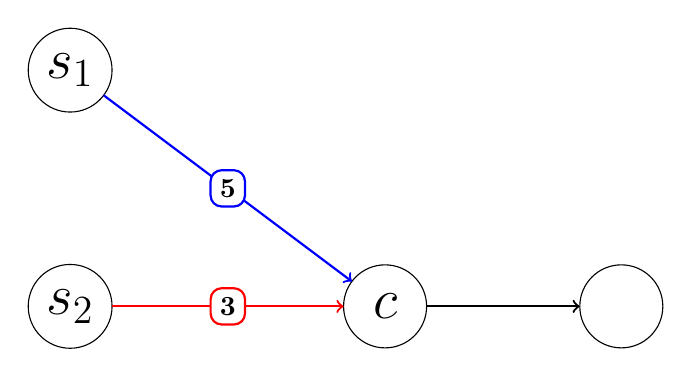
\begin{tikzpicture}
  \SetGraphUnit{5}
    \tikzset{
  EdgeStyle/.append style = {->} }
   \tikzstyle{VertexStyle}=[shape = circle, draw, minimum size = 30pt]
   \renewcommand{\VertexLightFillColor}{orange}
  \Vertex[x=0,y=3, L = {\huge $s_2$}]{a3};

  \Vertex[x=0,y=6, L = {\huge $s_1$}]{a1}


  \Vertex[x=4,y=3, L = {\huge $c$}]{c}

 \SetVertexNoLabel
\Vertex[x=7,y=3]{d}

      \Edge(c)(d)
  \tikzset{
  EdgeStyle/.append style = {blue} }
  \Edge[label = 5](a1)(c)   
 
  
    \tikzset{
  EdgeStyle/.append style = {red} }
    \Edge[label = 3](a3)(c)
  


\end{tikzpicture}
}
\end{center}

\end{frame}
 \begin{frame}{Collisions}

\begin{center}
\scalebox{0.6}{

\begin{tikzpicture}
  \SetGraphUnit{5}
    \tikzset{
  EdgeStyle/.append style = {->} }
   \tikzstyle{VertexStyle}=[shape = circle, draw, minimum size = 30pt]
   \renewcommand{\VertexLightFillColor}{orange}
  \Vertex[x=0,y=3, L = {\huge $s_2$}]{a3};

  \Vertex[x=0,y=6, L = {\huge $s_1$}]{a1}


  \Vertex[x=4,y=3, L = {\huge $c$}]{c}
   \draw[red] (4,3) circle (6ex);
 \SetVertexNoLabel
\Vertex[x=7,y=3]{d}

      \Edge(c)(d)
  \tikzset{
  EdgeStyle/.append style = {blue} }
  \Edge[label = 5](a1)(c)   
 
  
    \tikzset{
  EdgeStyle/.append style = {red} }
    \Edge[label = 3](a3)(c)
  
      
       \node (0) at (5,1){\includegraphics[scale=0.2]{col1.png}};


\end{tikzpicture}
}
\end{center}
\vspace{1cm}
\centering
There is a \textcolor{blue}{collision} between two routes when their messages go through the first vertex of a common arc at the same time.
\vspace{0.5cm}

 \textcolor{red}{Periodicity must be taken into consideration} 
\end{frame}



 \begin{frame}{Assignment }

 $P=13, \tau = 3$ 
 
\begin{center}
 \begin{multicols}{2}
\scalebox{0.6}{

\begin{tikzpicture}
  \SetGraphUnit{5}
    \tikzset{
  EdgeStyle/.append style = {->} }
   \tikzstyle{VertexStyle}=[shape = circle, draw, minimum size = 30pt]
   \renewcommand{\VertexLightFillColor}{orange}
  \Vertex[x=0,y=3, L = {\huge $s_2$}]{a3};

  \Vertex[x=0,y=6, L = {\huge $s_1$}]{a1}


  \Vertex[x=4,y=3, L = {\huge $c$}]{c}
  
 \SetVertexNoLabel
\Vertex[x=7,y=3]{d}

      \Edge(c)(d)

    
  \tikzset{
  EdgeStyle/.append style = {blue} }
  \Edge[label = 5](a1)(c)   
 
  
    \tikzset{
  EdgeStyle/.append style = {red} }
    \Edge[label = 3](a3)(c)
  \node (0) at (0,2.2){0};
      \node (0) at (0,5.2){0};
       \node (0) at (5,2){\includegraphics[scale=0.2]{col1.png}};


\end{tikzpicture}
}
\pause
\hspace{0.2cm}$\rightarrow$
\scalebox{0.6}{

\begin{tikzpicture}
  \SetGraphUnit{5}
    \tikzset{
  EdgeStyle/.append style = {->} }
   \tikzstyle{VertexStyle}=[shape = circle, draw, minimum size = 30pt]
   \renewcommand{\VertexLightFillColor}{orange}
  \Vertex[x=0,y=3, L = {\huge $s_2$}]{a3};

  \Vertex[x=0,y=6, L = {\huge $s_1$}]{a1}


  \Vertex[x=4,y=3, L = {\huge $c$}]{c}
  
 \SetVertexNoLabel
\Vertex[x=7,y=3]{d}

      \Edge(c)(d)

    
  \tikzset{
  EdgeStyle/.append style = {blue} }
  \Edge[label = 5](a1)(c)   
 
  
    \tikzset{
  EdgeStyle/.append style = {red} }
    \Edge[label = 3](a3)(c)
    \node (0) at (0,2.2){0};
      \node (0) at (0,5.2){1};
       \node (0) at (5,2){\includegraphics[scale=0.2]{col2.png}};


\end{tikzpicture}
}
\end{multicols}
\end{center}

\vspace{1cm}
\centering
Choosing the offset such that there are no collisions.
\vspace{0.5cm}
\pause

An \textcolor{blue}{assignment} is a choice of offsets for each route without collisions.
\end{frame}
\begin{frame}{Two way trip assignment}
 
 \begin{center}
\scalebox{0.3}{

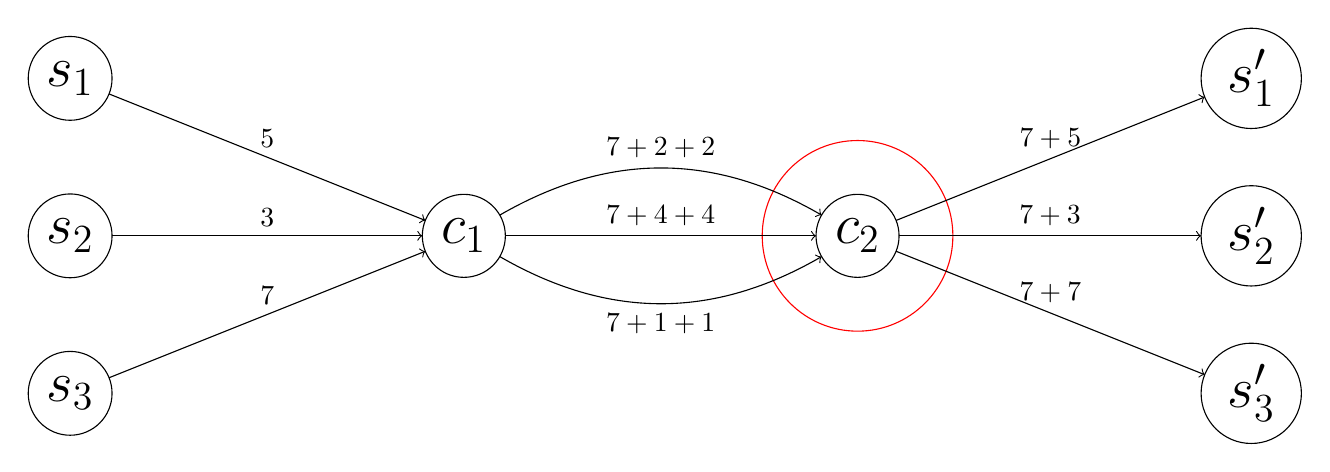
\begin{tikzpicture}
  \SetGraphUnit{5}
    \tikzset{
  EdgeStyle/.append style = {->} }
   \tikzstyle{VertexStyle}=[shape = circle, draw, minimum size = 30pt]
   \renewcommand{\VertexLightFillColor}{orange}
  \Vertex[x=0,y=4, L = {\huge $s_1$}]{s1};
  \Vertex[x=0,y=2, L = {\huge $s_2$}]{s2};
\Vertex[x=0,y=0, L = {\huge $s_3$}]{s3};
\Vertex[x=15,y=4, L = {\huge $s_1'$}]{s1p};
\Vertex[x=15,y=2, L = {\huge $s_2'$}]{s2p};
\Vertex[x=15,y=0, L = {\huge $s_3'$}]{s3p};
\draw[red] (10,2) circle (8ex);
\Vertex[x=10,y=2, L = {\huge $c_2$}]{c2};

  \Vertex[x=5,y=2, L = {\huge $c_1$}]{c1}
  
 %\SetVertexNoLabel
  %\Vertex[x=4,y=2]{n1}

  %\Edge[label = $5$](s1)(c1)
  %\Edge[label = $7 + 4+4$](c1)(c2)
  %\Edge[label = $3$](s2)(c1)
   %\Edge[label = $7$](s3)(c1)
  %  \Edge[label = $7+3$](c2)(s2p)
 %  \Edge[label = $7+7$](c2)(s3p)
%\Edge[label = $7 + 5$](c2)(s1p)
\path (s1) edge [->] node[anchor=south]{$5$} (c1);

\path (s2) edge [->] node[anchor=south]{$3$} (c1);
\path (s3) edge [->] node[anchor=south]{$7$} (c1);
\path (c2) edge [->] node[anchor=south]{$7+3$} (s2p);
\path (c2) edge [->] node[anchor=south]{$7+7$} (s3p);

\path (c2) edge [->] node[anchor=south]{$7+5$} (s1p);

\path (c1) edge [->] node[anchor=south]{$7+4+4$} (c2);

\path (c1) edge [->,bend left=30] node[anchor=south]{$7+2+2$} (c2);
\path (c1) edge [->,bend right=30] node[anchor=north]{$7+1+1$} (c2);

  %\draw[->,line width=0.5pt] (5,2.51) parabola bend (7.5,3.5) (10,2.51);
 %\draw[->,line width=0.5pt] (5,1.49) parabola bend (7.5,0.5) (10,1.49);
 

\end{tikzpicture}
}
\end{center}
\pause

In each BBU, one can choose the \textcolor{blue}{waiting time} before sending back the answer.\\

\begin{center}
  \includegraphics[scale=0.7]{BBU}\\
 \end{center} 

\pause
\todo{une figure pour expliquer ce que c'est un assignment (sur un graph on attend au debut et dans le point de la BBU)}
\textbf{Problem:}

Given a routed network, a period and a message size, find an assignment such that there is no collisions.
   
\end{frame}

\begin{frame}{Problems}
\textbf{Problem:}

Given a routed network, a period and a message size, find an assignment such that there is no collisions (PALL).
\textbf{Optimisation problem:}
Find an assignment that minimize the full process time.
\todo{une figure pour expliquer ce que c'est le full process time}

\textbf{Variant : PAZL}
No waiting time in the BBU.

\end{frame}


\begin{frame}{NP-hardness}

    \scalebox{0.5}{
    \begin{tikzpicture}
    \tikzset{
      LabelStyle/.style = { rectangle, rounded corners, draw,
        font = \bfseries },
    EdgeStyle/.append style = {->} }
      \SetGraphUnit{5}
      
  

      \tikzstyle{VertexStyle}=[shape = circle, draw, minimum size = 20pt]
  \tikzset{
   VertexStyle/.append style = {blue} }
  \Vertex[x=-8,y=3]{u}
        \tikzset{
      VertexStyle/.append style = {green} }
    \Vertex[x=-7,y=5]{v}

      \tikzset{
      VertexStyle/.append style = {red} }
    \Vertex[x=-6,y=4]{w}
    \tikzset{
      VertexStyle/.append style = {black} }
      
       
    
  \tikzset{
       EdgeStyle/.append style = {black,-} }

       \Edge(u)(v)
       \Edge(u)(w)
     \node (1) at (-3,4){\Huge $\rightarrow$};
      
     \node (2) at (-7,0){\Huge H};

     \end{tikzpicture}
     }

     Reduction of an instance H of vertex-coloring
\end{frame}
\begin{frame}{NP-hardness}

    \scalebox{0.5}{
    \begin{tikzpicture}
    \tikzset{
      LabelStyle/.style = { rectangle, rounded corners, draw,
        font = \bfseries },
    EdgeStyle/.append style = {->} }
      \SetGraphUnit{5}
      
      
      \node[draw,circle] (s3) at (4, 2) {$w^1$}; 
      \node[draw,circle] (s2) at (0, 4) {$v^1$}; 
      \node[draw,circle] (s1) at (0, 6) {$u^1$}; 

      \node[draw,circle] (t3) at (12, 3) {$w^2$}; 
      \node[draw,circle] (t2) at (10, 5) {$v^2$}; 
      \node[draw,circle] (t1) at (10, 2) {$u^2$}; 
      

      \tikzstyle{VertexStyle}=[shape = circle, draw, minimum size = 20pt]
  \tikzset{
   VertexStyle/.append style = {blue} }
  \Vertex[x=-8,y=3]{u}
        \tikzset{
      VertexStyle/.append style = {green} }
    \Vertex[x=-7,y=5]{v}

      \tikzset{
      VertexStyle/.append style = {red} }
    \Vertex[x=-6,y=4]{w}
    \tikzset{
      VertexStyle/.append style = {black} }
      
       
       \SetVertexNoLabel
       \Vertex[x=2,y=5]{A}


       \Vertex[x=6,y=3]{E}

       \tikzset{
       EdgeStyle/.append style = {green} }
       \Edge(s2)(A)
       
      \Edge(A)(t2)
 
       
       \tikzset{
      EdgeStyle/.append style = {red} }
       \Edge(s3)(E)
       \Edge(E)(t3) 
  \tikzset{
       EdgeStyle/.append style = {blue} }
       \Edge(s1)(A)
    
       \Edge(A)(E)
              
       \Edge(E)(t1)
       
  \tikzset{
       EdgeStyle/.append style = {black,-} }

       \Edge(u)(v)
       \Edge(u)(w)
     \node (1) at (-3,4){\Huge $\rightarrow$};
      
     \node (2) at (-7,0){\Huge H};
      \node (3) at (10,0){\Huge N};
     \end{tikzpicture}
     }

     Reduction of an instance H of vertex-coloring to an instance of PAZL.
\end{frame}
\section{Solving PALL on simple topologies (15 min)}
\subsection{Star shaped network}
\begin{frame}{Star Shaped network}
\begin{center}
\scalebox{0.4}{

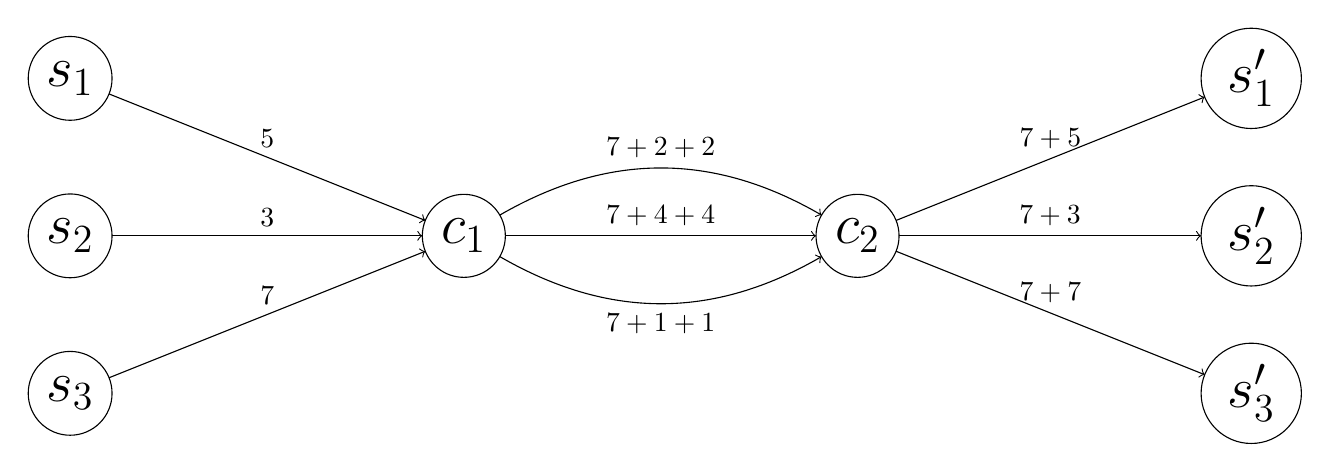
\begin{tikzpicture}
  \SetGraphUnit{5}
    \tikzset{
  EdgeStyle/.append style = {->} }
   \tikzstyle{VertexStyle}=[shape = circle, draw, minimum size = 30pt]
   \renewcommand{\VertexLightFillColor}{orange}
  \Vertex[x=0,y=4, L = {\huge $s_1$}]{s1};
  \Vertex[x=0,y=2, L = {\huge $s_2$}]{s2};
\Vertex[x=0,y=0, L = {\huge $s_3$}]{s3};
\Vertex[x=15,y=4, L = {\huge $s_1'$}]{s1p};
\Vertex[x=15,y=2, L = {\huge $s_2'$}]{s2p};
\Vertex[x=15,y=0, L = {\huge $s_3'$}]{s3p};
\Vertex[x=10,y=2, L = {\huge $c_2$}]{c2};

  \Vertex[x=5,y=2, L = {\huge $c_1$}]{c1}
  
 %\SetVertexNoLabel
  %\Vertex[x=4,y=2]{n1}

  %\Edge[label = $5$](s1)(c1)
  %\Edge[label = $7 + 4+4$](c1)(c2)
  %\Edge[label = $3$](s2)(c1)
   %\Edge[label = $7$](s3)(c1)
  %  \Edge[label = $7+3$](c2)(s2p)
 %  \Edge[label = $7+7$](c2)(s3p)
%\Edge[label = $7 + 5$](c2)(s1p)
\path (s1) edge [->] node[anchor=south]{$5$} (c1);

\path (s2) edge [->] node[anchor=south]{$3$} (c1);
\path (s3) edge [->] node[anchor=south]{$7$} (c1);
\path (c2) edge [->] node[anchor=south]{$7+3$} (s2p);
\path (c2) edge [->] node[anchor=south]{$7+7$} (s3p);

\path (c2) edge [->] node[anchor=south]{$7+5$} (s1p);

\path (c1) edge [->] node[anchor=south]{$7+4+4$} (c2);

\path (c1) edge [->,bend left=30] node[anchor=south]{$7+2+2$} (c2);
\path (c1) edge [->,bend right=30] node[anchor=north]{$7+1+1$} (c2);

  %\draw[->,line width=0.5pt] (5,2.51) parabola bend (7.5,3.5) (10,2.51);
 %\draw[->,line width=0.5pt] (5,1.49) parabola bend (7.5,0.5) (10,1.49);
 

\end{tikzpicture}
}

\pause
\vspace{1cm}
PAZL Solved for star shaped networks:
\begin{itemize}
	\item Fast greedy algorithms for light loads.
	\item FPT Algorithm for small number of routes.
	\end{itemize}
	\end{center}
\end{frame}
\subsection{A two stage approach for PALL}
\begin{frame}{A two stage approach for PALL}
\begin{center}
\textbf{First step:} We fix the offset of the route arbitrary.
\scalebox{0.4}{

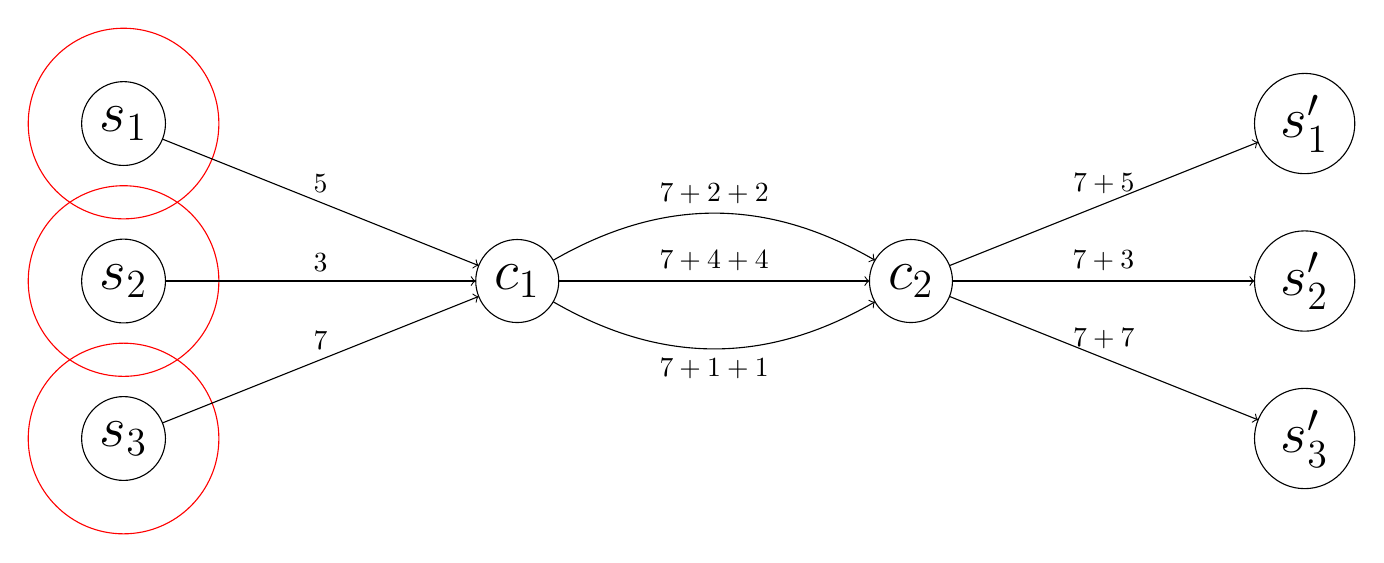
\begin{tikzpicture}
  \SetGraphUnit{5}
    \tikzset{
  EdgeStyle/.append style = {->} }
   \tikzstyle{VertexStyle}=[shape = circle, draw, minimum size = 30pt]
   \renewcommand{\VertexLightFillColor}{orange}
  \Vertex[x=0,y=4, L = {\huge $s_1$}]{s1};
  \Vertex[x=0,y=2, L = {\huge $s_2$}]{s2};
\Vertex[x=0,y=0, L = {\huge $s_3$}]{s3};
\Vertex[x=15,y=4, L = {\huge $s_1'$}]{s1p};
\Vertex[x=15,y=2, L = {\huge $s_2'$}]{s2p};
\Vertex[x=15,y=0, L = {\huge $s_3'$}]{s3p};
\Vertex[x=10,y=2, L = {\huge $c_2$}]{c2};
\draw[red] (0,0) circle (8ex);
\draw[red] (0,2) circle (8ex);
\draw[red] (0,4) circle (8ex);
  \Vertex[x=5,y=2, L = {\huge $c_1$}]{c1}
  
 %\SetVertexNoLabel
  %\Vertex[x=4,y=2]{n1}

  %\Edge[label = $5$](s1)(c1)
  %\Edge[label = $7 + 4+4$](c1)(c2)
  %\Edge[label = $3$](s2)(c1)
   %\Edge[label = $7$](s3)(c1)
  %  \Edge[label = $7+3$](c2)(s2p)
 %  \Edge[label = $7+7$](c2)(s3p)
%\Edge[label = $7 + 5$](c2)(s1p)
\path (s1) edge [->] node[anchor=south]{$5$} (c1);

\path (s2) edge [->] node[anchor=south]{$3$} (c1);
\path (s3) edge [->] node[anchor=south]{$7$} (c1);
\path (c2) edge [->] node[anchor=south]{$7+3$} (s2p);
\path (c2) edge [->] node[anchor=south]{$7+7$} (s3p);

\path (c2) edge [->] node[anchor=south]{$7+5$} (s1p);

\path (c1) edge [->] node[anchor=south]{$7+4+4$} (c2);

\path (c1) edge [->,bend left=30] node[anchor=south]{$7+2+2$} (c2);
\path (c1) edge [->,bend right=30] node[anchor=north]{$7+1+1$} (c2);

  %\draw[->,line width=0.5pt] (5,2.51) parabola bend (7.5,3.5) (10,2.51);
 %\draw[->,line width=0.5pt] (5,1.49) parabola bend (7.5,0.5) (10,1.49);
 

\end{tikzpicture}
}
 
 \pause
\textbf{Problem: Waiting Time Assignment:}
Given the offsets, the routed network and a deadline for all routes, find the assignment that minimize the full process time.

 \scalebox{0.4}{

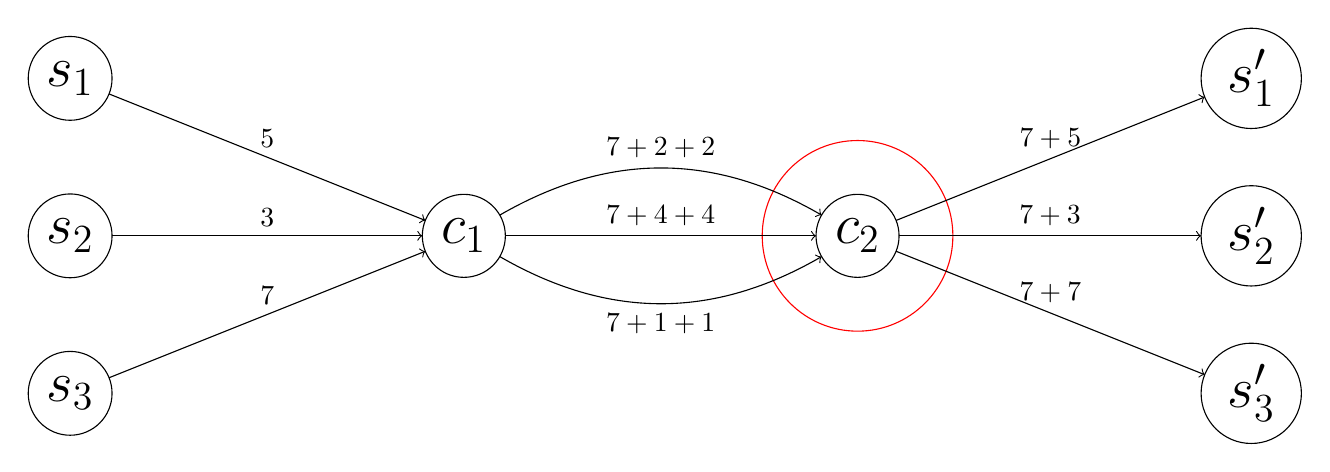
\begin{tikzpicture}
  \SetGraphUnit{5}
    \tikzset{
  EdgeStyle/.append style = {->} }
   \tikzstyle{VertexStyle}=[shape = circle, draw, minimum size = 30pt]
   \renewcommand{\VertexLightFillColor}{orange}
  \Vertex[x=0,y=4, L = {\huge $s_1$}]{s1};
  \Vertex[x=0,y=2, L = {\huge $s_2$}]{s2};
\Vertex[x=0,y=0, L = {\huge $s_3$}]{s3};
\Vertex[x=15,y=4, L = {\huge $s_1'$}]{s1p};
\Vertex[x=15,y=2, L = {\huge $s_2'$}]{s2p};
\Vertex[x=15,y=0, L = {\huge $s_3'$}]{s3p};
\Vertex[x=10,y=2, L = {\huge $c_2$}]{c2};

  \Vertex[x=5,y=2, L = {\huge $c_1$}]{c1}
  \draw[red] (10,2) circle (8ex);
 %\SetVertexNoLabel
  %\Vertex[x=4,y=2]{n1}

  %\Edge[label = $5$](s1)(c1)
  %\Edge[label = $7 + 4+4$](c1)(c2)
  %\Edge[label = $3$](s2)(c1)
   %\Edge[label = $7$](s3)(c1)
  %  \Edge[label = $7+3$](c2)(s2p)
 %  \Edge[label = $7+7$](c2)(s3p)
%\Edge[label = $7 + 5$](c2)(s1p)
\path (s1) edge [->] node[anchor=south]{$5$} (c1);

\path (s2) edge [->] node[anchor=south]{$3$} (c1);
\path (s3) edge [->] node[anchor=south]{$7$} (c1);
\path (c2) edge [->] node[anchor=south]{$7+3$} (s2p);
\path (c2) edge [->] node[anchor=south]{$7+7$} (s3p);

\path (c2) edge [->] node[anchor=south]{$7+5$} (s1p);

\path (c1) edge [->] node[anchor=south]{$7+4+4$} (c2);

\path (c1) edge [->,bend left=30] node[anchor=south]{$7+2+2$} (c2);
\path (c1) edge [->,bend right=30] node[anchor=north]{$7+1+1$} (c2);

  %\draw[->,line width=0.5pt] (5,2.51) parabola bend (7.5,3.5) (10,2.51);
 %\draw[->,line width=0.5pt] (5,1.49) parabola bend (7.5,0.5) (10,1.49);
 

\end{tikzpicture}
}
\end{center}
\end{frame}

\begin{frame}{Solving WTA: A greedy algorithm}

          \begin{center}
   \begin{tabularx}{0.7\textwidth}{|c|X|X|X|X|X|X|}
    \hline
     Route& $0$ & $1$ & $2$& $3$ & $4$\\
    \hline
    Deadline & $10$ &$15$&$5$&$7$&$30$\\
    \hline
     Release time & $0$ &$2$&$3$&$16$&$17$\\
    \hline
    Waiting time & $0$ &$5$&$1$&$0$&$15$\\
    \hline
      \end{tabularx}

\vspace{1cm}
      
       A run of GreedyDeadline with $P = 20, \tau = 4$.

      \includegraphics[width=0.7\textwidth]{greedy1.pdf}
\pause
\includegraphics[width=0.7\textwidth]{greedy2.pdf}
\pause
\includegraphics[width=0.7\textwidth]{greedy3.pdf}
\pause
\includegraphics[width=0.7\textwidth]{greedy4.pdf}
\pause
\includegraphics[width=0.7\textwidth]{greedy5.pdf}

 
      \end{center}
\end{frame}


\begin{frame}{Solving WTA: Polynomial time algorithms}

  
   \textbf{MLS} : Scheduling algorithm finding a solution minimizing makespawn. 
   \pause
   \textcolor{red}{Periodicity not managed.}      


   \pause 
   \textbf{PMLS} \todo{Une figure qui montre ce qui ne marcherais pas dans MLS et pourquoi PMLS trouve bcp plus d'instances}

   \textbf{ASPMLS} FPT-Algorithm based on PMLS $\rightarrow$ Always find the optimal solution when the number of routes is small.
\end{frame}



\subsection{Results}
\begin{frame}{Results: Algorithms for WTA}
\centering
\includegraphics[width=0.9\textwidth]{retour_21000.pdf}

\end{frame}
\begin{frame}{Results: PMLS against statistical multiplexing}
\centering
\includegraphics[width=\textwidth]{stochastic.pdf}
\end{frame}


\begin{frame}{Mixing C-RAN traffic with Best-Effort Traffic}
\centering
\includegraphics[width=0.9\textwidth]{res.pdf}

\end{frame}


\section{SPALL on random topologies (10 min)}
\subsection{Shape of the topologies(1min)}
\begin{frame}{Harder Instances}
\centering
%\includegraphics[width=0.9\textwidth]{graphmodel.pdf}
\scalebox{0.4}{

\begin{tikzpicture}
  \SetGraphUnit{5}
    \tikzset{
  EdgeStyle/.append style = {->} }
   \tikzstyle{VertexStyle}=[shape = circle, draw, minimum size = 30pt]
 

  \node (s8) at (0,10.5) {\includegraphics[width = 1cm]{rrh.png}};
  \node (s7) at (0,9) {\includegraphics[width = 1cm]{rrh.png}};
  \node (s6) at (0,7.5) {\includegraphics[width = 1cm]{rrh.png}};
  \node (s5) at (0,6) {\includegraphics[width = 1cm]{rrh.png}};
  \node (s4) at (0,4.5) {\includegraphics[width = 1cm]{rrh.png}};
  \node (s3) at (0,3) {\includegraphics[width = 1cm]{rrh.png}};
  \node (s2) at (0,1.5) {\includegraphics[width = 1cm]{rrh.png}};
  \node (s1) at (0,0) {\includegraphics[width = 1cm]{rrh.png}};
  
   \node (b2) at (10,7.25) {\includegraphics[width = 1cm]{bbu.png}};
   \node (b1) at (10,2.25) {\includegraphics[width = 1cm]{bbu.png}};

   \node (t6) at (8,7.25) {\includegraphics[width = 1cm]{switch.png}};
   \node (t5) at (8,2.25) {\includegraphics[width = 1cm]{switch.png}};
   \node (t4) at (4,9.75) {\includegraphics[width = 1cm]{switch.png}};
   \node (t3) at (4,6.75) {\includegraphics[width = 1cm]{switch.png}};
   \node (t2) at (4,3.75) {\includegraphics[width = 1cm]{switch.png}};
   \node (t1) at (4,0.75) {\includegraphics[width = 1cm]{switch.png}};

\path (s1) edge [<->,blue]  (t1);
\path (s2) edge [<->,green]  (t1);
\path (s3) edge [<->,red]  (t2);
\path (s4) edge [<->,orange]  (t2);
\path (s5) edge [<->,brown]  (t3);
\path (s6) edge [<->,purple]  (t3);
\path (s7) edge [<->,pink]  (t4);
\path (s8) edge [<->]  (t4);

\path (t1) edge [<->,blue]  (t5);
\path (t1) edge [<->,green]  (t6);
\path (t2) edge [<->,red]  (t5);
\path (t2) edge [<->,orange]  (t6);
\path (t3) edge [<->,brown]  (t5);
\path (t3) edge [<->,purple]  (t6);
\path (t4) edge [<->,pink]  (t5);
\path (t4) edge [<->]  (t6);

\path (t6) edge [<->,thick]  (b2);
\path (t5) edge [<->,thick]  (b1);


\node (k8) at (30,10.5) {$t_8$};
\node (k7) at (30,9) {$t_7$};
\node (k6) at (30,7.5) {$t_6$};
\node (k5) at (30,6) {$t_5$};
\node (k4) at (30,4.5) {$t_4$};
\node (k3) at (30,3) {$t_3$};
\node (k2) at (30,1.5) {$t_2$};
\node (k1) at (30,0) {$t_1$};

  \node (s8) at (14,10.5) {$s_8$};
  \node (s7) at (14,9) {$s_7$};
  \node (s6) at (14,7.5) {$s_6$};
  \node (s5) at (14,6) {$s_5$};
  \node (s4) at (14,4.5) {$s_4$};
  \node (s3) at (14,3) {$s_3$};
  \node (s2) at (14,1.5) {$s_2$};
  \node (s1) at (14,0) {$s_1$};


  
  \node (t10) at (26,9.75) {$c_{10}$};
   \node (t9) at (26,6.75) {$c_9$};
   \node (t8) at (26,3.75) {$c_8$};
   \node (t7) at (26,0.75) {$c_7$};
   \node (t6) at (22,7.25) {$c_6$};
   \node (t5) at (22,2.25) {$c_5$};
   \node (t4) at (18,9.75) {$c_4$};
   \node (t3) at (18,6.75) {$c_3$};
   \node (t2) at (18,3.75) {$c_2$};
   \node (t1) at (18,0.75) {$c_1$};

\path (s1) edge [->,blue]  (t1);
\path (s2) edge [->,green]  (t1);
\path (s3) edge [->,red]  (t2);
\path (s4) edge [->,orange]  (t2);
\path (s5) edge [->,brown]  (t3);
\path (s6) edge [->,purple]  (t3);
\path (s7) edge [->,pink]  (t4);
\path (s8) edge [->]  (t4);

\path (t1) edge [->,blue]  (t5);
\path (t1) edge [->,green]  (t6);
\path (t2) edge [->,red]  (t5);
\path (t2) edge [->,orange]  (t6);
\path (t3) edge [->,brown]  (t5);
\path (t3) edge [->,purple]  (t6);
\path (t4) edge [->,pink]  (t5);
\path (t4) edge [->]  (t6);

\path (k1) edge [->,blue]  (t7);
\path (k2) edge [->,green]  (t7);
\path (k3) edge [->,red]  (t8);
\path (k4) edge [->,orange]  (t8);
\path (k5) edge [->,brown]  (t9);
\path (k6) edge [->,purple]  (t9);
\path (k7) edge [->,pink]  (t10);
\path (k8) edge [->]  (t10);

\path (t7) edge [->,blue]  (t5);
\path (t7) edge [->,green]  (t6);
\path (t8) edge [->,red]  (t5);
\path (t8) edge [->,orange]  (t6);
\path (t9) edge [->,brown]  (t5);
\path (t9) edge [->,purple]  (t6);
\path (t10) edge [->,pink]  (t5);
\path (t10) edge [->]  (t6);




\end{tikzpicture}
}



\end{frame}
\begin{frame}{Greedy Dealine}
\begin{center}
	\includegraphics[width=\linewidth]{examplegreedyfail}
	\end{center}
\end{frame}
\begin{frame}{Greedy Packed}
\begin{center}
	Slide avec le même exemple mais greedy packed.
	\end{center}
\end{frame}
\begin{frame}{Performance of greedy algorithms}

      \begin{minipage}[b]{0.49\linewidth}
   \includegraphics[width=\linewidth]{90load.pdf}
  \end{minipage} 
  \begin{minipage}[b]{0.49\linewidth}
      \includegraphics[width=\linewidth]{greedysuccess.pdf}
  \end{minipage} 
\end{frame}






\subsection{Compact form}
\begin{frame}{Compact representation}
\begin{center}
	\includegraphics[width=\linewidth]{normalizedassignment}
	\end{center}
\end{frame}
\begin{frame}{Assignment from a compact representation }
\begin{center}
	\includegraphics[width=\linewidth]{compacttoassignment}

	Inductive construction of an assignment from the compact assignment $((2,1,0,3),\{1\})$ on a single contention point .
\end{center}
\end{frame}
\subsection{Local search algorithms }
\begin{frame}{Local Search Algorithms}

   \textbf{Hill Climbing} : Starting from Hybrid Greedy Normalized
   \pause
 
   \textbf{Tabu Search} Long computation time, not efficient
\pause
   \textbf{Simulated Annealing} Solutions close to the optimal solutions. Complexity : exponential in the contention depth.
\pause
   \textbf{Branch and Bound algorithm} Exponential in the number of routes and the contention depth.

\end{frame}
\subsection{Results}
\begin{frame}{Results}
\begin{center}
	\includegraphics[width=\linewidth]{all8routes}

\end{center}
\end{frame}
\section{Conclusion}
\begin{frame}{Conclusion}

   \begin{itemize}
   	\item An industrial prototype in development.
   	\item Hot topic in telecommunications.
   	\item 2 registered patents.
   \end{itemize}


   \begin{itemize}
   	\item 2 International publications \todo{citer?}.
   	\item Complexification of the model: 
   	\begin{itemize}
   		\item Different link size.
   		\item Not the same period for all messages.
   		\item Different message size.
   	\end{itemize}
   	\item 1 Journal paper submitted.
   	\item 2 Articles beeing finalized.
   \end{itemize}
\end{frame}





\end{document}
